\documentclass[../../Thesis.tex]{subfiles}
\begin{document}
\header{Data}
\subheader{Corpus}
The dataset we used for this research consists of all articles\footnote{From Elseviers corpus} published in 2017 which have been published in a journal that has, in 2017, atleast 150 publications. This results in a total dataset of $1.391.543$ articles from $3.759$ journals.
\begin{table}[hbt]
\begin{center}
\begin{tabular}{|l|c|c|c|c|}
\hline
 & Total word count & Unique word count & Total token count & Unique token count \\
\hline
Title & $18.822.399$ & $939.665$ & $14.742.192$ & $230.805$ \\
\hline
Abstract & $264.653.020$ & $5.853.077$ & $171.474.473$ & $738.961$ \\
\hline
Total & $283.475.419$ & $6.209.769$ & $186.962.354$ & $763.475$ \\
\hline
\end{tabular}
\end{center}
\caption{Corpus size}\label{table:corpusSize}
\end{table}\\
The word occurrences follow the pattern of a pareto distribution as described by~\citet{wiegand2018word}. This distribution is visualized in XXXXXX, which displays the occurrences of the first 500 tokens of the corpus.
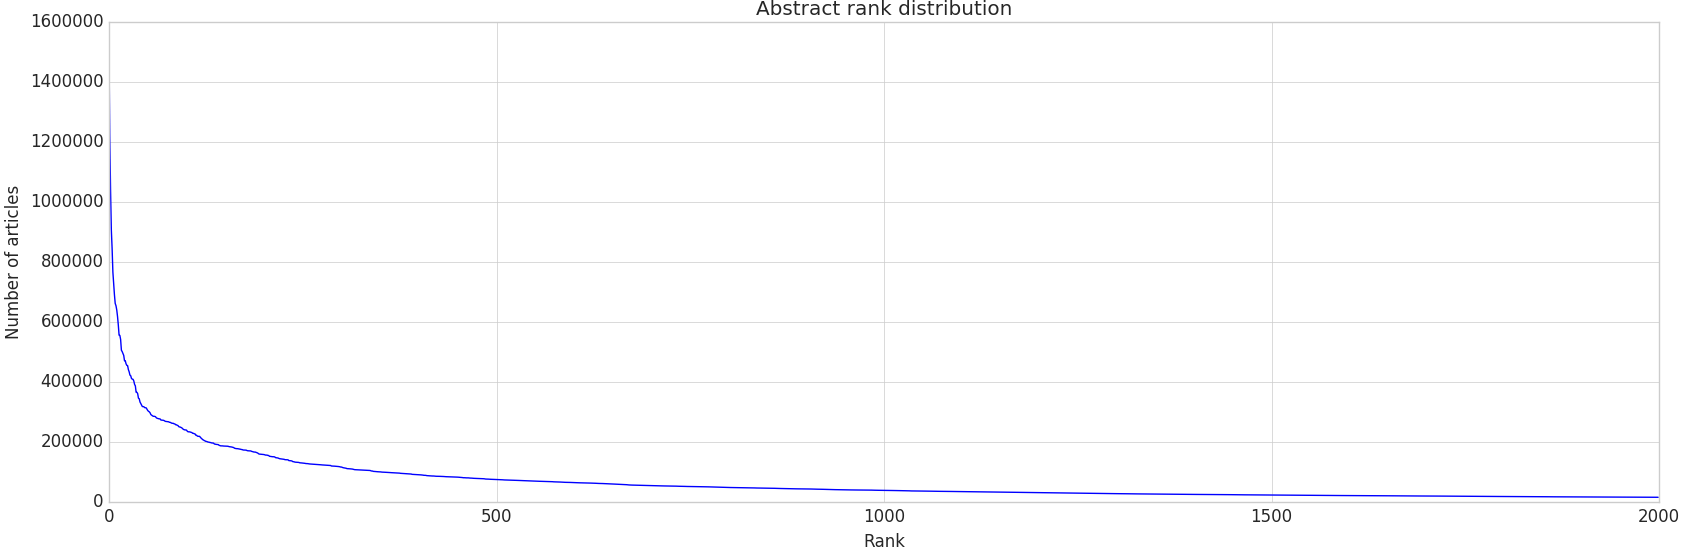
\includegraphics[width=6.5in]{Plots/word_occurrences}\\

\subheader{Datasets}
For this researched we used a (pre-made) tokenized dataset, which reduces the total amount of words by 34\%, from this tokenized set, we created the embeddings and the TF-IDF feature vectors.
\subsubheader{Tokenization}
The following steps have been applied to the words to create a tokenized set:
\begin{enumerate}
\item{Removed punctuation}
\item{Removed all non-ascii characters}
\item{Transformed all characters to lower-case}
\item{Removed stop-words, as provided by the NLTK library}
\item{Removed numbers}
\item{Stemmed all words, using the stemmer provided by the NLTK library}
\end{enumerate}
These transformations reduced our dataset by 34\%, resulting in a tokenized set of $186.962.354$ tokens.

\subsubheader{Embedding}
For this research we reused the word embeddings created by \citet{Truong2017Thesis}. These embeddings have a vector size of 300, which is an industry default. They have been trained on the entire Elsevier corpus, not limited to the subset we used for this research. To construct article embeddings we take the average of all normalized word embeddings for that article. Journal embeddings are constructed in the same way, we averaged all the normalized article embeddings to create the journal embeddings. We have used multiple embedding configurations for this research
\subsubsubheader{Default embedding}
The default embedding is created form the pre-trained word embeddings, no modifications have been applied to this set.
\subsubsubheader{TF-IDF embedding}
The TF-IDF weighted embedding set, referred to as TF-IDF embedding, are the default word embeddings weighted with a TF-IDF score per word.\\
The TF-IDF is calculated with a raw token count, and a smoothed inverted document frequency, calculated as follows:\\
\begin{equation}
IDF = \log_{10}(\dfrac{|A|}{|A_t|})
\end{equation}
Where $|A|$ is the total count of articles and $|A_t|$ is the count of articles containing term t.
The articles embeddings are a normalized summation of each word vector multiplied by it TF-IDF value. Since we take a sum of all words, the Term Frequency is embedded as the raw count of each word.
\subsubsubheader{10K TF-IDF embedding}
The 10K embedding set is generated similarity to the TF-IDF embedding, this version only uses the 10.000 most common tokens, reducing the amount of tokens it uses. This set was created to see if the limitation to 10.000 tokens reduces the amount of noise, and with that increasing the performance.
\subsubsubheader{5K TF-IDF embedding}
The 5K TF-IDF embedding is the TF-IDF embedding set, limited to the 5.000 most common words. This set was created to more aggressively limit the amount of tokens, and with that, cancel out more noise.
\subsubsubheader{1K-6K TF-IDF embedding}
The 1K-6K TF-IDF embedding is the TF-IDF embedding limited to the top 6.000 most common words, without the top 1.000 most common words. The rationale for this is that common words will occur in many articles, creating noise, by cutting of the top 1.000 and cutting of everything below 6.000 we tried to reduce the noise by filtering common words. This cut results in a set of 5.000 tokens, which allows us to compare it to the 5K TF-IDF set.

\subsubheader{TF-IDF}
To create the TF-IDF feature vectors, we used the TF-IDF model and a hasher from pysparks the MlLib library. The TF-IDF feature vectors are created by hashing the tokens with the hasher, which has a set hash bucket size. These hashed values are passed on to the TF-IDF model, resulting in a feature vector which vector dimensions equals the amount of hash buckets. To limit the computational and storage expenses and to reduce noise by rare words, we limit our vocabulary size.
We denote the TF-IDF configurations as follows: $vocabulary size/hashbucket size$. Furthermore, we denote 1.000 as 1K, since we deal with chosen values which can be exactly noted given this notation.\\
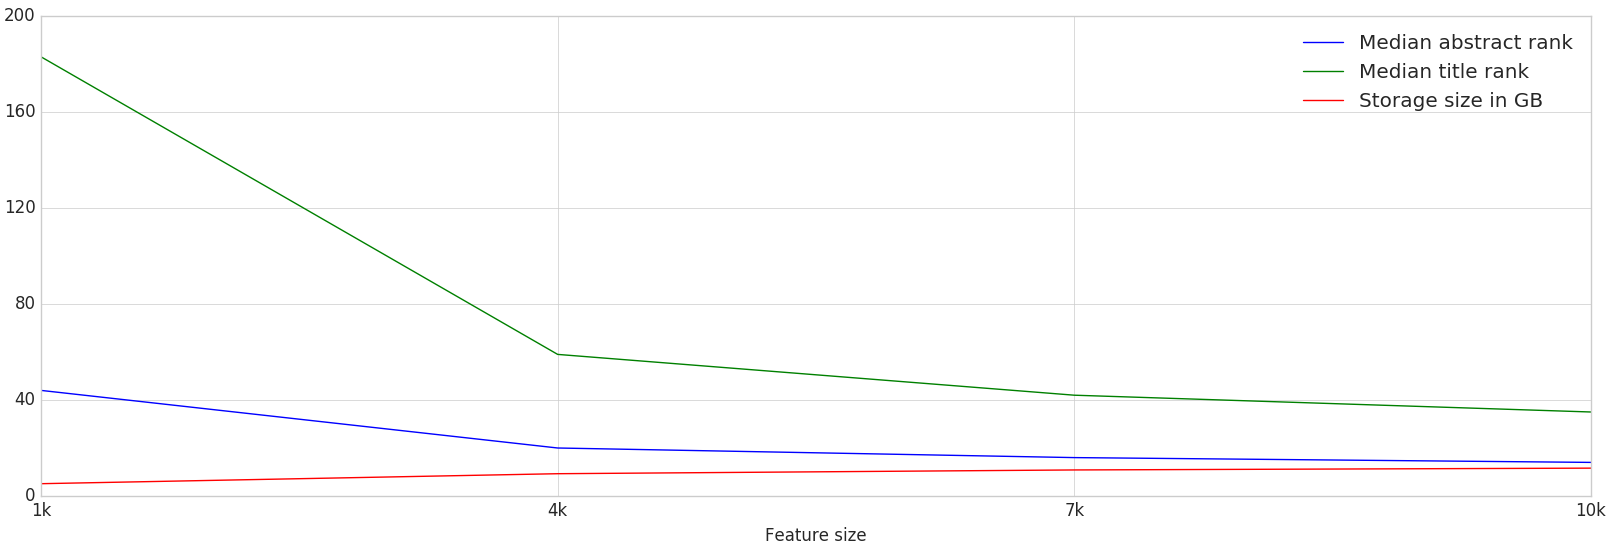
\includegraphics[width=6in]{Plots/tfidf_selection_plot}\\
The graph XXX shows the performance and storage size\footnote{in gigabyte, 1024 based} of the 1k/1K, 4K/4K, 7K/7K and 10K/10K TF-IDF configurations. This plot shows that, while the required storage size keeps rising, the performance on title quickly stagnates, and the performance on abstract follows too. Given this information, we have chosen to use the 10K/10K, 10K/5K and 5K/5K configurations to compare our embedding results to.

\end{document}

% RAW DATA:
% 1,391,543 articles
% 14 811 433 title tokens			230805 unique		18.822.399			939.665
% 172 150 921 abstract tokens		738961 unique		264.653.020			5.853.077
% 186 962 354 total tokens			763475 unique		283.475.419			6.209.769
% 3,759 journals

% split = 79.9509609117 - 20.0490390883

% training numbers
% 10K = percentage?}